\section{Analisi tramite calcolo matriciale}
Come prima operazione è stato definito il vettore degli spostamenti:
\[
\overline{u}^T = \left[u_1,v_1,\varphi_1,u_2,v_2,\varphi_2,\varphi_2^{EF5},u_3,v_3^{EF2},v_3^{EF3},\varphi_3^{EF2},\varphi_3^{EF3},u_4,v_4,\varphi_4,u_5,v_5,\varphi_5 \right]
\]
Si sono quindi definite le matrici di assemblaggio e di rotazione per ciascun elemento.
%
%Matrici di assemblaggio
%
\begin{align*}
\mathbf{A_1} &=
{\arraycolsep=1pt\medmuskip=0.8mu\footnotesize
\left[
\begin{array}{cccccccccccccccccc}
 1 & 0 & 0 & 0 & 0 & 0 & 0 & 0 & 0 & 0 & 0 & 0 & 0 & 0 & 0 & 0 & 0 & 0 \\
 0 & 1 & 0 & 0 & 0 & 0 & 0 & 0 & 0 & 0 & 0 & 0 & 0 & 0 & 0 & 0 & 0 & 0 \\
 0 & 0 & 1 & 0 & 0 & 0 & 0 & 0 & 0 & 0 & 0 & 0 & 0 & 0 & 0 & 0 & 0 & 0 \\
 0 & 0 & 0 & 1 & 0 & 0 & 0 & 0 & 0 & 0 & 0 & 0 & 0 & 0 & 0 & 0 & 0 & 0 \\
 0 & 0 & 0 & 0 & 1 & 0 & 0 & 0 & 0 & 0 & 0 & 0 & 0 & 0 & 0 & 0 & 0 & 0 \\
 0 & 0 & 0 & 0 & 0 & 1 & 0 & 0 & 0 & 0 & 0 & 0 & 0 & 0 & 0 & 0 & 0 & 0 \\
 \end{array}
 \right]
 }
\qquad
 \mathbf{A_2} =
{\arraycolsep=1pt\medmuskip=0.8mu\footnotesize
\left[
\begin{array}{cccccccccccccccccc}
 0 & 0 & 0 & 1 & 0 & 0 & 0 & 0 & 0 & 0 & 0 & 0 & 0 & 0 & 0 & 0 & 0 & 0 \\
 0 & 0 & 0 & 0 & 1 & 0 & 0 & 0 & 0 & 0 & 0 & 0 & 0 & 0 & 0 & 0 & 0 & 0 \\
 0 & 0 & 0 & 0 & 0 & 1 & 0 & 0 & 0 & 0 & 0 & 0 & 0 & 0 & 0 & 0 & 0 & 0 \\
 0 & 0 & 0 & 0 & 0 & 0 & 0 & 1 & 0 & 0 & 0 & 0 & 0 & 0 & 0 & 0 & 0 & 0 \\
 0 & 0 & 0 & 0 & 0 & 0 & 0 & 0 & 1 & 0 & 0 & 0 & 0 & 0 & 0 & 0 & 0 & 0 \\
 0 & 0 & 0 & 0 & 0 & 0 & 0 & 0 & 0 & 0 & 1 & 0 & 0 & 0 & 0 & 0 & 0 & 0 \\
 \end{array}
 \right]
 }
 \\
 \mathbf{A_3} &=
{\arraycolsep=1pt\medmuskip=0.8mu\footnotesize
\left[
\begin{array}{cccccccccccccccccc}
 0 & 0 & 0 & 0 & 0 & 0 & 0 & 1 & 0 & 0 & 0 & 0 & 0 & 0 & 0 & 0 & 0 & 0 \\
 0 & 0 & 0 & 0 & 0 & 0 & 0 & 0 & 0 & 1 & 0 & 0 & 0 & 0 & 0 & 0 & 0 & 0 \\
 0 & 0 & 0 & 0 & 0 & 0 & 0 & 0 & 0 & 0 & 0 & 1 & 0 & 0 & 0 & 0 & 0 & 0 \\
 0 & 0 & 0 & 0 & 0 & 0 & 0 & 0 & 0 & 0 & 0 & 0 & 1 & 0 & 0 & 0 & 0 & 0 \\
 0 & 0 & 0 & 0 & 0 & 0 & 0 & 0 & 0 & 0 & 0 & 0 & 0 & 1 & 0 & 0 & 0 & 0 \\
 0 & 0 & 0 & 0 & 0 & 0 & 0 & 0 & 0 & 0 & 0 & 0 & 0 & 0 & 1 & 0 & 0 & 0 \\
 \end{array}
 \right]
 } 
 \qquad
 \mathbf{A_4} =
{\arraycolsep=1pt\medmuskip=0.8mu\footnotesize
\left[
\begin{array}{cccccccccccccccccc}
 0 & 0 & 0 & 0 & 0 & 0 & 0 & 0 & 0 & 0 & 0 & 0 & 1 & 0 & 0 & 0 & 0 & 0 \\
 0 & 0 & 0 & 0 & 0 & 0 & 0 & 0 & 0 & 0 & 0 & 0 & 0 & 1 & 0 & 0 & 0 & 0 \\
 0 & 0 & 0 & 0 & 0 & 0 & 0 & 0 & 0 & 0 & 0 & 0 & 0 & 0 & 1 & 0 & 0 & 0 \\
 0 & 0 & 0 & 0 & 0 & 0 & 0 & 0 & 0 & 0 & 0 & 0 & 0 & 0 & 0 & 1 & 0 & 0 \\
 0 & 0 & 0 & 0 & 0 & 0 & 0 & 0 & 0 & 0 & 0 & 0 & 0 & 0 & 0 & 0 & 1 & 0 \\
 0 & 0 & 0 & 0 & 0 & 0 & 0 & 0 & 0 & 0 & 0 & 0 & 0 & 0 & 0 & 0 & 0 & 1 \\
 \end{array}
 \right]
 }
\\
 \mathbf{A_5} &=
{\arraycolsep=1pt\medmuskip=0.8mu\footnotesize
\left[
\begin{array}{cccccccccccccccccc}
 0 & 0 & 0 & 0 & 0 & 0 & 0 & 0 & 0 & 0 & 0 & 0 & 0 & 0 & 0 & 1 & 0 & 0 \\
 0 & 0 & 0 & 0 & 0 & 0 & 0 & 0 & 0 & 0 & 0 & 0 & 0 & 0 & 0 & 0 & 1 & 0 \\
 0 & 0 & 0 & 0 & 0 & 0 & 0 & 0 & 0 & 0 & 0 & 0 & 0 & 0 & 0 & 0 & 0 & 1 \\
 0 & 0 & 0 & 1 & 0 & 0 & 0 & 0 & 0 & 0 & 0 & 0 & 0 & 0 & 0 & 0 & 0 & 0 \\
 0 & 0 & 0 & 0 & 1 & 0 & 0 & 0 & 0 & 0 & 0 & 0 & 0 & 0 & 0 & 0 & 0 & 0 \\
 0 & 0 & 0 & 0 & 0 & 0 & 1 & 0 & 0 & 0 & 0 & 0 & 0 & 0 & 0 & 0 & 0 & 0 \\
 \end{array}
 \right]
 }
 \end{align*}%
%
%Matrici di rotazione
%
\begin{align*}
\mathbf{T_1}=\mathbf{T(0)} &=
{\arraycolsep=3pt\medmuskip=0.8mu\footnotesize
\left[
\begin{array}{cccccc}
 1 & 0 & 0 & 0 & 0 & 0 \\
 0 & 1 & 0 & 0 & 0 & 0 \\
 0 & 0 & 1 & 0 & 0 & 0 \\
 0 & 0 & 0 & 1 & 0 & 0 \\
 0 & 0 & 0 & 0 & 1 & 0 \\
 0 & 0 & 0 & 0 & 0 & 1 \\
\end{array}
 \right]
 }
\qquad
\mathbf{T_2}=\mathbf{T(-\pi/2)} =
{\arraycolsep=3pt\medmuskip=0.8mu\footnotesize
\left[
\begin{array}{cccccc}
 0 & -1 & 0 & 0 & 0 & 0 \\
 1 & 0 & 0 & 0 & 0 & 0 \\
 0 & 0 & 1 & 0 & 0 & 0 \\
 0 & 0 & 0 & 0 & -1 & 0 \\
 0 & 0 & 0 & 1 & 0 & 0 \\
 0 & 0 & 0 & 0 & 0 & 1 \\
\end{array}
 \right]
 }
 \\
 \mathbf{T_3}=\mathbf{T(0)} &=
{\arraycolsep=3pt\medmuskip=0.8mu\footnotesize
\left[
\begin{array}{cccccc}
 1 & 0 & 0 & 0 & 0 & 0 \\
 0 & 1 & 0 & 0 & 0 & 0 \\
 0 & 0 & 1 & 0 & 0 & 0 \\
 0 & 0 & 0 & 1 & 0 & 0 \\
 0 & 0 & 0 & 0 & 1 & 0 \\
 0 & 0 & 0 & 0 & 0 & 1 \\
\end{array}
 \right]
 } 
 \qquad
 \mathbf{T_4}=\mathbf{T(\pi/2)} =
{\arraycolsep=3pt\medmuskip=0.8mu\footnotesize
\left[
\begin{array}{cccccc}
 0 & -1 & 0 & 0 & 0 & 0 \\
 1 & 0 & 0 & 0 & 0 & 0 \\
 0 & 0 & 1 & 0 & 0 & 0 \\
 0 & 0 & 0 & 0 & -1 & 0 \\
 0 & 0 & 0 & 1 & 0 & 0 \\
 0 & 0 & 0 & 0 & 0 & 1 \\
\end{array}
 \right]
 }
\\
\mathbf{T_5}=\mathbf{T\Big(\pi/2 + \arctan(2)\Big)} &=
{\arraycolsep=3pt\medmuskip=0.8mu\footnotesize
\left[
\begin{array}{cccccc}
 -\frac{2}{\sqrt{5}} & \frac{1}{\sqrt{5}} & 0 & 0 & 0 & 0 \\
 -\frac{1}{\sqrt{5}} & -\frac{2}{\sqrt{5}} & 0 & 0 & 0 & 0 \\
 0 & 0 & 1 & 0 & 0 & 0 \\
 0 & 0 & 0 & -\frac{2}{\sqrt{5}} & \frac{1}{\sqrt{5}} & 0 \\
 0 & 0 & 0 & -\frac{1}{\sqrt{5}} & -\frac{2}{\sqrt{5}} & 0 \\
 0 & 0 & 0 & 0 & 0 & 1 \\
\end{array}
\right]
 }
 \end{align*}
 Sono state poi definite la matrice di rigidezza della molla e il vettore dei carichi nodali.
 %
%Matrice molla
%
\[
\mathbf{K_{molla}} =
{\arraycolsep=2pt\medmuskip=0.8mu\footnotesize
\left[
\begin{array}{cccccccccccccccccc}
 0 & 0 & 0 & 0 & 0 & 0 & 0 & 0 & 0 & 0 & 0 & 0 & 0 & 0 & 0 & 0 & 0 & 0 \\
 0 & 0 & 0 & 0 & 0 & 0 & 0 & 0 & 0 & 0 & 0 & 0 & 0 & 0 & 0 & 0 & 0 & 0 \\
 0 & 0 & 0 & 0 & 0 & 0 & 0 & 0 & 0 & 0 & 0 & 0 & 0 & 0 & 0 & 0 & 0 & 0 \\
 0 & 0 & 0 & 0 & 0 & 0 & 0 & 0 & 0 & 0 & 0 & 0 & 0 & 0 & 0 & 0 & 0 & 0 \\
 0 & 0 & 0 & 0 & 0 & 0 & 0 & 0 & 0 & 0 & 0 & 0 & 0 & 0 & 0 & 0 & 0 & 0 \\
 0 & 0 & 0 & 0 & 0 & 0 & 0 & 0 & 0 & 0 & 0 & 0 & 0 & 0 & 0 & 0 & 0 & 0 \\
 0 & 0 & 0 & 0 & 0 & 0 & 0 & 0 & 0 & 0 & 0 & 0 & 0 & 0 & 0 & 0 & 0 & 0 \\
 0 & 0 & 0 & 0 & 0 & 0 & 0 & k & 0 & 0 & 0 & 0 & 0 & 0 & 0 & 0 & 0 & 0 \\
 0 & 0 & 0 & 0 & 0 & 0 & 0 & 0 & 0 & 0 & 0 & 0 & 0 & 0 & 0 & 0 & 0 & 0 \\
 0 & 0 & 0 & 0 & 0 & 0 & 0 & 0 & 0 & 0 & 0 & 0 & 0 & 0 & 0 & 0 & 0 & 0 \\
 0 & 0 & 0 & 0 & 0 & 0 & 0 & 0 & 0 & 0 & 0 & 0 & 0 & 0 & 0 & 0 & 0 & 0 \\
 0 & 0 & 0 & 0 & 0 & 0 & 0 & 0 & 0 & 0 & 0 & 0 & 0 & 0 & 0 & 0 & 0 & 0 \\
 0 & 0 & 0 & 0 & 0 & 0 & 0 & 0 & 0 & 0 & 0 & 0 & 0 & 0 & 0 & 0 & 0 & 0 \\
 0 & 0 & 0 & 0 & 0 & 0 & 0 & 0 & 0 & 0 & 0 & 0 & 0 & 0 & 0 & 0 & 0 & 0 \\
 0 & 0 & 0 & 0 & 0 & 0 & 0 & 0 & 0 & 0 & 0 & 0 & 0 & 0 & 0 & 0 & 0 & 0 \\
 0 & 0 & 0 & 0 & 0 & 0 & 0 & 0 & 0 & 0 & 0 & 0 & 0 & 0 & 0 & 0 & 0 & 0 \\
 0 & 0 & 0 & 0 & 0 & 0 & 0 & 0 & 0 & 0 & 0 & 0 & 0 & 0 & 0 & 0 & 0 & 0 \\
 0 & 0 & 0 & 0 & 0 & 0 & 0 & 0 & 0 & 0 & 0 & 0 & 0 & 0 & 0 & 0 & 0 & 0 \\
\end{array}
\right]
}
\]
%
%Forze nodali
%
\[
\overline{R} = \overline{R}_V + \overline{R}_Q +\overline{R}_P +\overline{R}_T =
%
{\arraycolsep=2pt\medmuskip=0.8mu\footnotesize
\left[
\begin{array}{c}
    H1\\V1\\M1\\0\\0\\0\\0\\0\\0\\0\\0\\0\\0\\0\\0\\0\\0\\0    
\end{array}\right]
+
\left[
\begin{array}{c}
    0\\0\\0\\0\\0\\0\\0\\0\\0\\\frac{QL}{2}\\0\\\frac{QL^2 }{12}\\0\\\frac{QL}{2}\\-\frac{QL^2}{12}\\0\\0\\0    
\end{array}\right]
+
\left[
\begin{array}{c}
    0\\0\\0\\0\\0\\0\\0\\0\\0\\0\\0\\0\\0\\0\\0\\0\\F\\0    
\end{array}\right]
+\left[
\begin{array}{c}
    0\\0\\\frac{2 EI\alpha \Delta T}{h}\\0\\0\\-\frac{2EI\alpha \Delta T} {h}\\0\\0\\0\\0\\0\\0\\0\\0\\0\\0\\0\\0   
\end{array}\right]
}
\]
Infine si è calcolata la matrice di rigidezza globale totale -- riportata a pagina \pageref{MatriceKtot} --  riducendola poi in base alle condizioni al contorno essenziali omogenee. 
Risolvendo il sistema e sostituendo i valori del problema, si sono ottenuti i risultati riportati nei vettori $\overline{u}$ e $\overline{R}_V$ a pagina \pageref{vet:UeRV}. 
 %%%%%%%%%%%%%%%%%%%%%%%%%%%%%%%%%%%%%%%%%%%%%%%%%
 %Matrice globale senza numeri
\begin{landscape}
\begin{figure}[htb]
    \centering
    {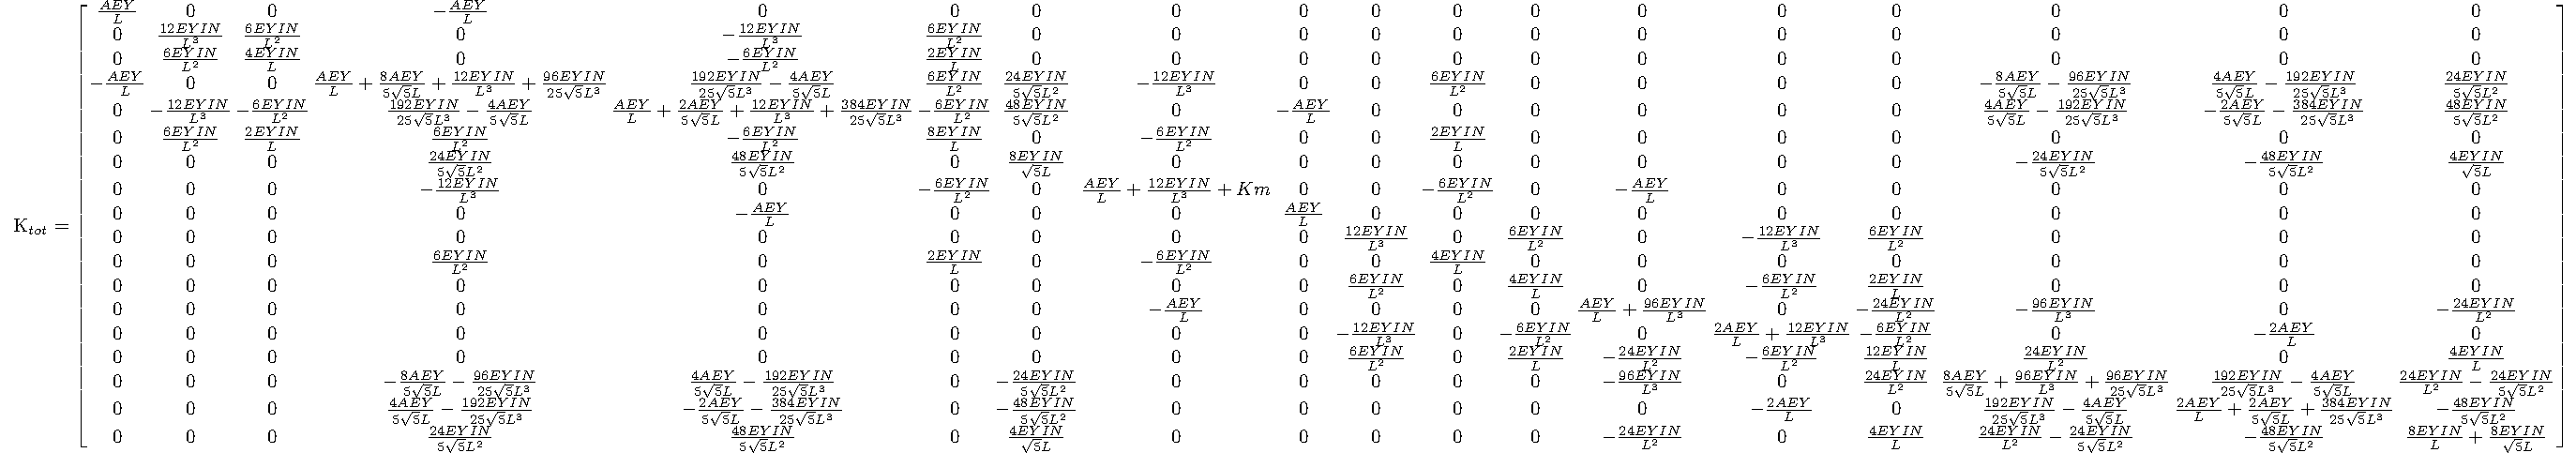
\includegraphics[width=20cm,trim=0 0 23.5cm 0,clip]{rel1/img1/ktot.pdf}}\\  
    
    \vspace{1cm}
    {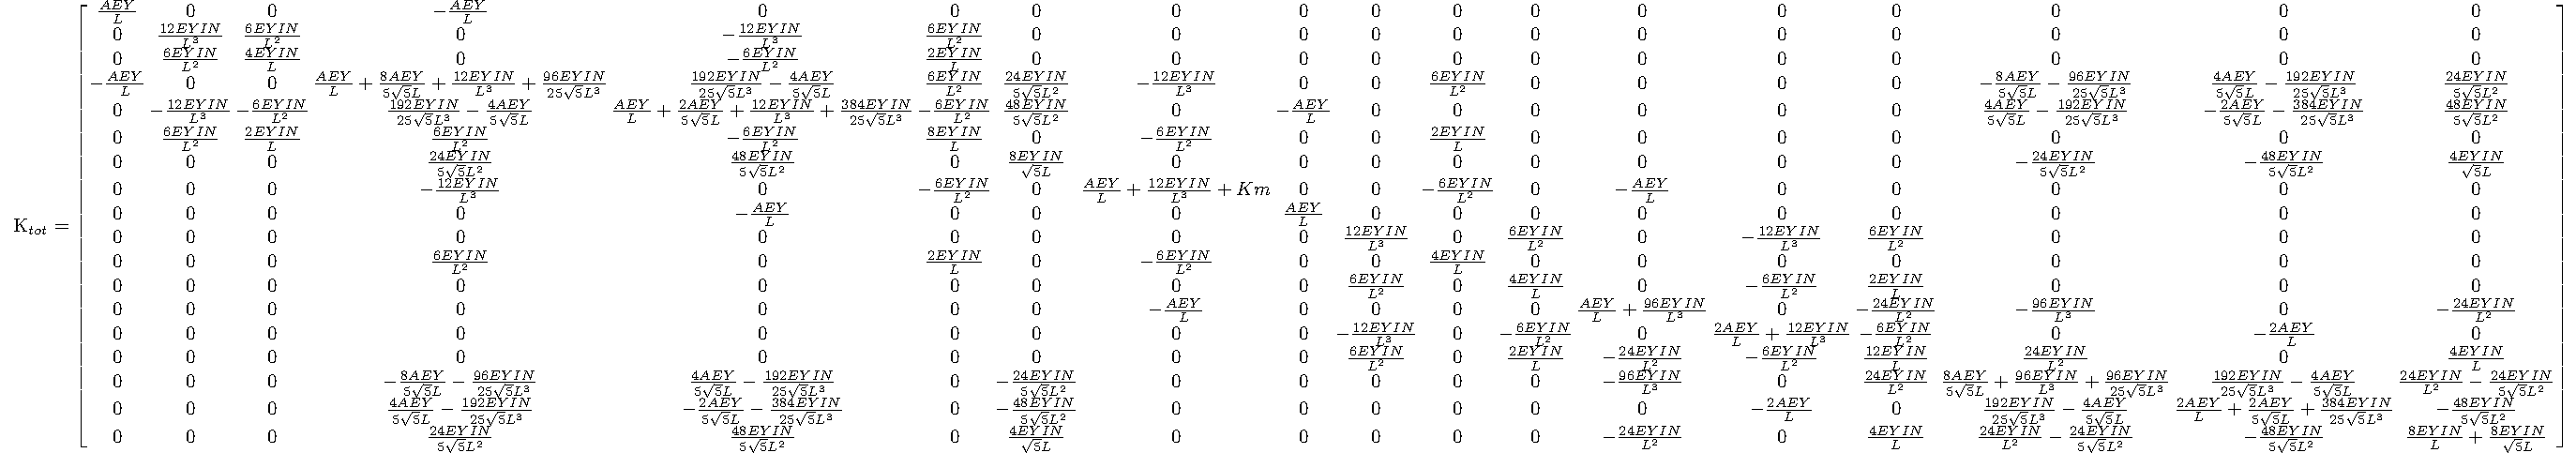
\includegraphics[width=19cm,trim=23cm 0 0 0,clip]{rel1/img1/ktot.pdf}}
    \label{MatriceKtot}
\end{figure}
\end{landscape}
%Risultati U e RV
\[
\label{vet:UeRV}
\overline{u} = \left[
    \begin{array}{c}
    0\\0\\0\\\SI{-7.22e-7}{}\\\SI{6.31e-4}{}\\\SI{3.32e-3}{}\\\SI{8.37e-3}{}\\\SI{4.31e-3}{}\\\SI{6.31e-4}{}\\\SI{3.80e-2}{}\\\SI{3.81e-3}{}\\\SI{-7.35e-3}{}\\\SI{4.32e-3}{}\\\SI{1.76e-2}{}\\\SI{-5.11e-3}{}\\\SI{8.47e-3}{}\\\SI{1.76e-2}{}\\\SI{2.22e-4}{}
    \end{array}
    \right]
\qquad    
\overline{R}_V = \left[
    \begin{array}{c}
    96.07\\\SI{-1.500e3}{}\\\SI{-7.362e3}{}\\0\\0\\0\\0\\0\\0\\0\\0\\0\\0\\0\\0\\0\\0\\0 
    \end{array}
    \right]
\]
